\section{Additional results}
\label{app:extra}
\begin{table}[h]\centering\footnotesize
\caption{Closed-form leverage vs simulation (E1, \textsc{ols-s}). Runs are (setting, world) pairs. Left: simulated mean leverage over $R$ assignments divided by $L$ of Prop.~\ref{prop:lev}; right: observed RMSE divided by $\hat\kappa\sqrt{L/n}$ (median [min, max]).}
\label{tab:lev}\begin{tabular}{lrcc}\toprule
family/design & runs & $\bar L_{\rm sim}/L$ & RMSE / predicted \\
\midrule
BA/Bern. & 24 & 1.01 [1.00, 1.02] & 1.01 [0.91, 1.05] \\
BA/cluster & 24 & 1.40 [1.10, 2.33] & 1.23 [0.90, 1.66] \\
ER/Bern. & 72 & 1.01 [1.00, 1.07] & 1.01 [0.89, 1.10] \\
SBM/Bern. & 30 & 1.01 [1.00, 1.04] & 1.00 [0.92, 1.10] \\
SBM/cluster & 30 & 1.36 [1.12, 2.65] & 1.20 [0.85, 1.75] \\
Stanford3/Bern. & 6 & 1.00 [1.00, 1.00] & 1.03 [0.98, 1.09] \\
Stanford3/cluster & 24 & 1.15 [1.05, 15.57] & 1.11 [0.77, 3.74] \\
WS/Bern. & 24 & 1.01 [1.00, 1.03] & 1.00 [0.91, 1.08] \\
WS/cluster & 24 & 1.03 [1.03, 1.04] & 1.00 [0.85, 1.19] \\
ego-Facebook/Bern. & 6 & 1.02 [1.02, 1.02] & 1.05 [0.85, 1.13] \\
ego-Facebook/cluster & 24 & 1.07 [1.03, 1.30] & 1.08 [0.69, 1.50] \\
\bottomrule\end{tabular}\end{table}

\begin{table}[h]\centering\footnotesize
\caption{Dependence on the baseline scale $\sigma_a$ (E1; ER, $n=4000$, $d=16$, Bernoulli; effect heterogeneity fixed at $0.5$).}
\label{tab:siga}\begin{tabular}{rrr}\toprule
$\sigma_a$ & RMSE & bias \\
\midrule
0.25 & 0.065 & -0.002 \\
0.50 & 0.085 & +0.004 \\
1.00 & 0.132 & +0.003 \\
2.00 & 0.254 & -0.004 \\
4.00 & 0.503 & -0.002 \\
\bottomrule\end{tabular}\end{table}

\begin{table}[h]\centering\footnotesize
\caption{Clustering quality and error (E5, linear response, \textsc{ols-s}, $p=\frac12$): number of Louvain clusters, fraction of edges cut, simulated mean leverage, closed-form leverage, RMSE (means over 6 worlds).}
\label{tab:clu}\begin{tabular}{lrrrrr}\toprule
graph & clusters & cut & $\bar L_{\rm sim}$ & $L$ & RMSE \\
\midrule
SBM & 6 & 0.44 & 72.3 & 13.7 & 0.120 \\
SBM & 10 & 0.50 & 61.6 & 21.5 & 0.146 \\
SBM & 21 & 0.55 & 55.5 & 31.7 & 0.140 \\
SBM & 40 & 0.57 & 54.4 & 40.5 & 0.124 \\
SBM & 83 & 0.63 & 43.5 & 35.9 & 0.117 \\
SBM & 154 & 0.75 & 51.8 & 45.7 & 0.131 \\
SBM & 324 & 0.84 & 72.5 & 67.3 & 0.148 \\
SBM & 690 & 0.89 & 91.1 & 87.5 & 0.166 \\
Stanford3 & 5 & 0.02 & 461.3 & 4.3 & 0.151 \\
Stanford3 & 9 & 0.34 & 56.2 & 7.3 & 0.066 \\
Stanford3 & 18 & 0.53 & 14.1 & 10.4 & 0.035 \\
Stanford3 & 42 & 0.61 & 14.8 & 12.6 & 0.038 \\
Stanford3 & 76 & 0.67 & 15.4 & 13.9 & 0.040 \\
Stanford3 & 155 & 0.72 & 16.5 & 15.4 & 0.043 \\
Stanford3 & 288 & 0.76 & 17.6 & 16.7 & 0.044 \\
Stanford3 & 621 & 0.81 & 20.4 & 19.8 & 0.045 \\
ego-Facebook & 7 & 0.00 & 6.6 & 4.1 & 0.049 \\
ego-Facebook & 11 & 0.03 & 5.5 & 4.3 & 0.042 \\
ego-Facebook & 19 & 0.06 & 5.3 & 4.6 & 0.040 \\
ego-Facebook & 44 & 0.32 & 5.9 & 5.5 & 0.043 \\
ego-Facebook & 92 & 0.41 & 6.2 & 5.8 & 0.043 \\
ego-Facebook & 172 & 0.49 & 6.7 & 6.4 & 0.043 \\
ego-Facebook & 310 & 0.58 & 7.4 & 7.1 & 0.045 \\
ego-Facebook & 559 & 0.70 & 9.0 & 8.7 & 0.052 \\
\bottomrule\end{tabular}\end{table}

\begin{table}[t]\centering\footnotesize
\caption{Crossover spillover strength $\gamma^\ast$ above which the one-hop regression has lower RMSE than DiM (E4; ER graphs, Bernoulli; $\beta\approx1$), versus $\hat\kappa\sqrt{L/n}$; RMSE of DiM and regression at $\gamma=0$. H\'ajek (E1, $n=4000$) is undefined in a fraction 0.00, 0.00, 0.79, 1.00, 1.00, 1.00, 1.00 of draws for $d=4,8,16,32,64,128,256$ respectively.}
\label{tab:cross}\begin{tabular}{rrrrrr}\toprule
$d$ & $n$ & $\gamma^\ast$ (obs.) & $\hat\kappa\sqrt{L/n}$ & DiM RMSE & reg. RMSE \\
\midrule
8 & 1000 & 0.174 & 0.199 & 0.064 & 0.190 \\
8 & 4000 & 0.088 & 0.099 & 0.033 & 0.095 \\
8 & 16000 & 0.033 & 0.050 & 0.016 & 0.047 \\
32 & 1000 & 0.372 & 0.402 & 0.064 & 0.376 \\
32 & 4000 & 0.181 & 0.201 & 0.032 & 0.191 \\
32 & 16000 & 0.094 & 0.100 & 0.017 & 0.094 \\
128 & 1000 & 0.823 & 0.805 & 0.067 & 0.822 \\
128 & 4000 & 0.387 & 0.402 & 0.032 & 0.380 \\
128 & 16000 & 0.191 & 0.201 & 0.016 & 0.187 \\
\bottomrule\end{tabular}\end{table}


\paragraph{Notes.} (i) In Table~\ref{tab:lev} the closed-form leverage is essentially exact for Bernoulli designs (within $7\%$ in every run, within $2\%$ in the median family) and underestimates the simulated leverage for cluster designs, by a median of $3$--$40\%$ per family and by a factor up to $15.6$ (Stanford3 with 9 clusters), consistent with Prop.~\ref{prop:lev} being an expectation over assignments. (ii) In Table~\ref{tab:clu} the closed-form leverage is accurate once there are about $\ge20$ clusters. (iii) Table~\ref{tab:siga}: RMSE scales sublinearly in $\sigma_a$ because effect heterogeneity (coefficients $\beta_i,\gamma_i$ with 50\% relative SD) adds a baseline-independent component.

\begin{table}[t]\centering\footnotesize\setlength{\tabcolsep}{3.5pt}
\caption{Nonlinear exposure response (E2): bias (RMSE) of the GATE estimate; true GATE $\approx2$. Mean over 6 worlds ($R{=}300$). $^\dagger$ \textsc{gbm}: 3 worlds, $R{=}40$ assignments each. ``--'': H\'ajek undefined in $\ge50\%$ of draws (or not run).}
\label{tab:extrap}
\begin{tabular}{lllccccc}\toprule
graph & response & design & \textsc{ols-s} & +$s^2$ & +$s^2,s^3$ & \textsc{gbm}$^\dagger$ & H\'ajek \\
\midrule
ER & k=4 & Bern. & -0.45 (0.50) & -0.45 (0.50) & +0.01 (1.92) & -0.65 (0.83) & -- \\
 &  & cluster & -0.36 (0.52) & -0.45 (0.54) & +0.03 (1.51) & -0.60 (0.72) & -- \\
 & threshold & Bern. & +1.46 (1.48) & +1.47 (1.49) & -2.34 (3.06) & -0.14 (0.52) & -- \\
 &  & cluster & +0.94 (1.02) & +1.48 (1.52) & -0.65 (2.27) & -0.08 (0.41) & -- \\
ego-Facebook & k=4 & Bern. & -0.22 (0.30) & -0.24 (0.27) & -0.01 (0.17) & -0.17 (0.49) & -0.01 (0.65) \\
 &  & cluster & -0.03 (0.08) & -0.03 (0.06) & +0.00 (0.05) & -0.01 (0.22) & -0.00 (0.07) \\
 & threshold & Bern. & +0.60 (0.61) & +0.64 (0.66) & -0.07 (0.18) & +0.12 (0.41) & -0.01 (0.63) \\
 &  & cluster & +0.05 (0.07) & +0.05 (0.07) & -0.01 (0.05) & -0.01 (0.25) & -0.00 (0.07) \\
Stanford3 & k=4 & Bern. & -0.13 (0.15) & -0.13 (0.15) & -0.01 (0.08) & -0.26 (0.37) & -0.01 (0.50) \\
 &  & cluster & -0.12 (0.21) & -0.13 (0.14) & -0.00 (0.06) & -0.11 (0.21) & -0.00 (0.17) \\
 & threshold & Bern. & +0.37 (0.37) & +0.37 (0.37) & -0.03 (0.09) & -0.11 (0.26) & -0.03 (0.48) \\
 &  & cluster & +0.20 (0.20) & +0.23 (0.24) & -0.06 (0.08) & -0.06 (0.14) & +0.00 (0.16) \\
\bottomrule\end{tabular}\end{table}

\begin{table}[t]\centering\footnotesize\setlength{\tabcolsep}{3.5pt}
\caption{Multi-hop spillover, $\lambda=0.6$ (E3): bias (RMSE) of DiM, one-hop regression and regression with two-step exposure; last two columns: closed-form bias of the one-hop regression under Bernoulli designs (exact walk-statistics formula, tree-like approximation). Mean over 6 worlds.}
\label{tab:mh}
\begin{tabular}{llccccc}\toprule
graph/design & GATE & DiM & \textsc{ols-s} & \textsc{ols-s2} & $B$ exact & $B$ tree \\
\midrule
ER/Bern. & 2.49 & -1.48 (1.48) & -0.87 (0.89) & -0.55 (1.19) & -0.867 & -0.900 \\
SBM/Bern. & 2.49 & -1.49 (1.49) & -0.86 (0.88) & -0.48 (1.16) & -- & -0.900 \\
SBM/cluster & 2.49 & -1.15 (1.15) & -0.67 (0.69) & -0.43 (0.83) & -- & -- \\
ego-FB/Bern. & 2.49 & -1.47 (1.47) & -0.71 (0.76) & -0.22 (0.65) & -0.696 & -0.900 \\
ego-FB/cluster & 2.49 & -0.34 (0.35) & -0.11 (0.16) & -0.02 (0.13) & -- & -- \\
Stanford3/Bern. & 2.50 & -1.49 (1.49) & -0.85 (0.85) & -0.42 (0.55) & -0.850 & -0.900 \\
Stanford3/cluster & 2.50 & -1.01 (1.01) & -0.49 (0.50) & -0.20 (0.23) & -- & -- \\
\bottomrule\end{tabular}\end{table}


\begin{figure}[h]
\centering
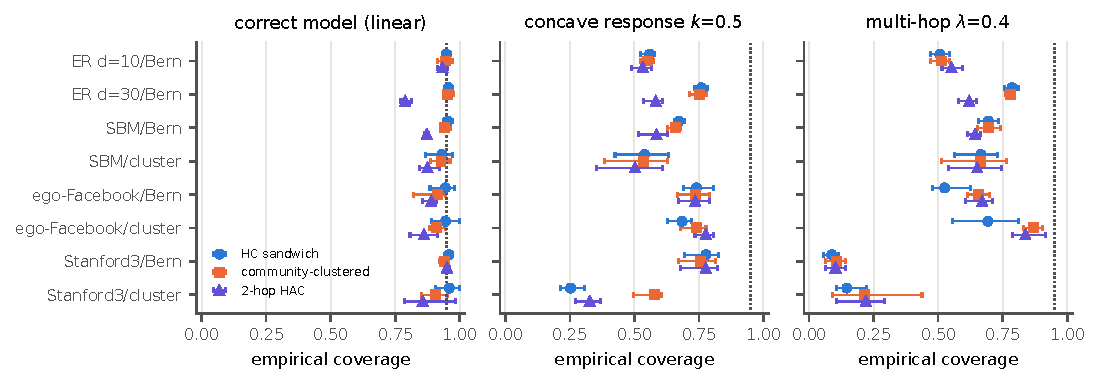
\includegraphics[width=\linewidth]{figs/fig_inference.pdf}
\caption{Coverage of nominal 95\% intervals for the one-hop regression estimator (E6). Markers: mean over 6 worlds; bars min--max. Dotted: 0.95.}
\label{fig:inf}
\end{figure}

\begin{figure}[h]
\centering
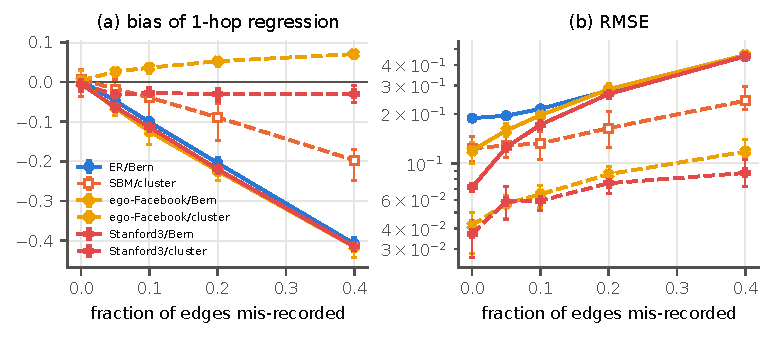
\includegraphics[width=0.62\linewidth]{figs/fig_obsnoise.pdf}
\caption{Mis-measured network (E7): (a) bias and (b) RMSE of the one-hop regression vs fraction of edges replaced by random edges (mean over 6 worlds; bars min--max).}
\label{fig:obs}
\end{figure}


\section{Reproducibility details}
\label{app:repro}
\textbf{Code and instructions.} All code, raw results (CSV), logs and this paper's source are in the released archive; \texttt{README.md} gives the full procedure and \texttt{run\_all\_experiments.sh} runs it end to end. \textbf{Environment:} Python 3.11.2; numpy 2.4.6, scipy 1.17.1, networkx 3.6.1, pandas 3.1.1, scikit-learn 1.9.1, matplotlib 3.11.2 (\texttt{requirements.txt}); pdfLaTeX (TeX Live) with the official \texttt{neurips\_2026.sty}. \textbf{Hardware/time:} CPU only; the container was limited to 4 CPU cores (cgroup quota) with 251\,GB RAM available (memory use was not profiled; each worker held at most one graph and, for E6's HAC, one $\approx10^7$--$10^8$-entry sparse matrix). Wall-clock times of the final runs on 4 processes: E1 172\,s, E2 473\,s, E2g (boosting) 181\,s, E3 355\,s, E4 177\,s, E5 1269\,s, E6 858\,s, E7 64\,s, exact walk statistics (\texttt{psi.py}) $\approx4$\,min; about $1$\,h in total ($\approx4$ CPU-hours); the 3-world pilot of E1/E3 cost a few minutes.
\textbf{Data.} Stanford3: \url{https://nrvis.com/download/data/socfb/socfb-Stanford3.zip} (Network Repository, CC BY-SA; original source Traud et al.~\citep{traud2012social}; file \texttt{socfb-Stanford3.mtx}, $11586\times11586$, 568{,}309 edges; zip SHA-256 \texttt{b1221e41\ldots e8720d}, verified, 1{,}649{,}740 bytes). ego-Facebook: \url{https://snap.stanford.edu/data/facebook_combined.txt.gz} (SNAP; McAuley and Leskovec~\citep{mcauley2012learning}; 88{,}234 edges, 4{,}039 nodes; SHA-256 \texttt{125e84db\ldots 35d7}, verified, 218{,}576 bytes). Downloads are parsed as plain text only (never executed) by \texttt{code/graphs.py}; both graphs are connected so the largest-component restriction is the identity. Synthetic graphs use \texttt{networkx}.
\textbf{Seeds.} Synthetic graph of world $i$: seed $100+i$; outcome parameters of world $i$: seed $1000+i$ ($i=0..5$); the assignment RNG of each configuration is seeded by the first 8 hex digits of the SHA-256 of its (graph, mechanism, design, $i$) description (\texttt{experiments.stable\_seed}); Louvain clustering uses seed 1 (cached on disk for the real graphs). We re-ran E7 and obtained bit-identical numeric output (the other experiments use the same mechanism; they were not re-run end to end).
\textbf{Script $\to$ output.} Fig.~1 \texttt{fig\_variance.py} (E1); Fig.~2 \texttt{fig\_extrap.py} (E2; $\hat\kappa$ from \texttt{stats\_summary.py}); Fig.~3 \texttt{fig\_multihop.py} (E3, \texttt{psi.py}); Fig.~4 \texttt{fig\_crossover.py} (E4); Fig.~5 \texttt{fig\_design.py} (E5); Figs.~6--7 \texttt{fig\_inference.py}, \texttt{fig\_obsnoise.py} (E6, E7); Table~1 \texttt{mk\_tables.py:tab\_het} (E3); Tables~2--7 \texttt{mk\_tables.py} (E1--E5); every number quoted in the text is printed by \texttt{stats\_summary.py} or \texttt{verify\_claims.py}. \textbf{Literature access.} Only the starter literature and unrelated public papers were consulted (searches by title for the cited works). No page matching the withheld paper was knowingly opened; a few search-result titles/abstract snippets of unrelated network-interference papers were seen incidentally and none was read further.
